\documentclass[12pt]{article}
\usepackage{graphicx}
\usepackage{amsmath}
\usepackage{listings}
\usepackage{authblk}
\usepackage{geometry}
\usepackage{hyperref,xcolor}
\usepackage{float}
\geometry{margin=1in}

\begin{document}

\title{AI-Assisted Teacher Professional Development in Peru: Analyzing Classroom Observations with the World Bank TEACH Framework}
\author[1]{Matthew D.\ Krasnow}
\author[2]{Ezequiel Molina}
\author[2]{Carolina Lopez}
\author[3]{Carolina Moreira Vasquez}
\author[1]{Will Krasnow}

\affil[1]{SwiftScore\\ \texttt{\{matt, will\} @swiftscore.org}}
\affil[2]{World Bank\\ \texttt{\{molina, carolina\_lopez\}@worldbank.org}}
\affil[3]{University of Virginia\\ \texttt{cmm9mn@virginia.edu}}

\date{}
\maketitle

\begin{abstract}
\noindent \textbf{Abstract.} This paper examines an AI-driven approach to teacher professional development using classroom observation data from Peru. We situate our work in the context of global teacher shortages and uneven instructional quality, highlighting the potential for artificial intelligence (AI) to scale support for teachers. Using the World Bank’s \textit{TEACH} framework for classroom observations, we detail a methodology that begins with raw video data and ends with automated teaching evaluations. Video recordings of lessons (two per classroom session) are algorithmically assigned, converted to audio, and transcribed with a state-of-the-art speech-to-text system. We clean the transcripts and pair them with human-coded observation scores in order to train and evaluate AI models. Our evaluation centers on how closely the AI’s ratings of teaching practices align with human evaluators at both the component and domain levels. We define a distance-based accuracy metric and conduct a Monte Carlo simulation of the World Bank’s teacher reliability certification exam to assess whether the AI can meet the rigorous criteria for “reliable” observers. Results show that with a well-designed rubric and transcript processing, the AI achieves high agreement with human scores—e.g., a refined rubric model passes 89.3\% of classroom segments, versus 70.2\% for a baseline model. We integrate visualizations illustrating domain-level accuracy and certification outcomes. We discuss the implications of these findings for integrating AI into teacher professional development infrastructure, noting potential policy benefits in scaling teacher support alongside cautionary considerations for ethical deployment.
\end{abstract}

\section{Introduction}
\label{sec:intro}
\noindent Around the world, education systems are grappling with severe teacher shortages and uneven teaching quality. UNESCO estimates that by 2030 the world will need approximately 44 million additional primary and secondary teachers to meet global education goals. In sub-Saharan Africa alone, 15 million new teachers are needed, and even high-income regions struggle to recruit and retain qualified educators. These shortages exacerbate large class sizes and undermine instructional quality, contributing to a global learning crisis. As of 2023, seven in ten children in low- and middle-income countries could not read and understand a simple text by age 10, a stark indicator of how gaps in teacher supply and support translate into poor learning outcomes. Ensuring students receive quality instruction from well-prepared teachers is essential for improving these outcomes, yet many classrooms—especially in underserved areas—lack access to ongoing teacher coaching and feedback.

Meanwhile, advances in artificial intelligence (AI) offer new avenues to support teachers at scale. AI applications in education have shown promise in aiding instruction and professional development by providing on-demand feedback, automating administrative tasks, and facilitating personalized coaching. For example, recent studies demonstrate that AI-driven professional development programs can help teachers adopt more effective pedagogical practices, leading to measurably improved instruction quality. AI tutors and virtual coaches can deliver “just-in-time” feedback to teachers, simulating some benefits of in-person mentoring in a scalable, accessible manner. These developments suggest that AI might play a key role in alleviating the twin challenges of teacher shortages and uneven training, by augmenting (though not replacing) human-led professional development.

In this context, our work explores an AI-assisted approach to teacher evaluation and feedback, focusing on data from Peru’s teacher professional development program. Peru faces significant educational challenges common to many countries: ensuring high-quality teaching in every classroom despite resource constraints and varying teacher skill levels. The dataset used in this study consists of classroom observation sessions collected as part of the World Bank’s \textit{TEACH} program in Peru. \textit{TEACH} is a standardized classroom observation tool that “captures teaching practices that support quality learning, considering time spent on learning as well as the quality of teaching practices.” It provides a structured rubric and protocol for observers to score a lesson on multiple domains of teacher practice. By leveraging this framework, we aim to train AI models that can evaluate teaching in alignment with expert human observers, thus serving as a virtual coach or co-observer in the professional development process.

This paper presents a comprehensive pipeline and evaluation of such AI models, with the Peru dataset as a case study. In Section 2, we review the dataset and our methodology, including how raw classroom videos were processed into text transcripts and paired with human scoring data. Section 3 details how we evaluated the AI’s performance using the TEACH rubric—covering distance-based accuracy calculations, inter-rater reliability measures, and a simulated certification exam to test whether the AI meets the criteria for reliable observers. In Section 4, we present results, including visualizations of domain-level accuracy and the AI models’ pass/fail rates under exam conditions. Section 5 discusses the implications of these findings: we examine how rubric design and data preparation affected performance, the potential of AI to fill gaps in teacher coaching, and cautionary notes on ensuring such systems are used constructively. Finally, Section 6 concludes with recommendations for integrating AI into teacher professional development and considerations for policymakers looking to harness AI while upholding teaching standards and ethics.

\section{Methodology}
\label{sec:methods}
\subsection{Dataset and Preprocessing}
\noindent \textbf{Peru Classroom Observation Data.} The study utilizes a dataset of teacher classroom observations collected in Peru in 2019 as part of a World Bank education project. Each observation consists of a classroom session (approximately 30 minutes in total) that was originally captured in multiple video clips. The accompanying data file contains human evaluator scores for each session across the TEACH rubric components (detailed below). We began by consolidating and preprocessing this raw data. A key initial step was the \textit{video discovery and assignment}: mapping the multiple video files to each observation and selecting the appropriate clips for analysis. In the Peru dataset, each classroom session could have been recorded in up to 3 or 4 separate clips due to camera limitations. We identified that out of 363 total observation entries, 17 had no video available and 100 had only one clip. Those sessions were omitted from further analysis since the TEACH protocol requires two observation segments per lesson. For sessions with 3 or 4 clips, we applied a heuristic to choose the most pertinent footage: using file timestamps, we selected the first and last clips as representative bookends of the lesson, discarding intermediate clips. This yielded a refined set of 246 observation sessions (67.8\% of the total) with exactly two video clips each.

\textbf{Audio Conversion.} To facilitate automated transcription, the video clips were converted to audio format (MP3). We developed an optimized multi-threaded pipeline for this conversion, taking advantage of available GPU hardware for acceleration where possible. The conversion process was designed to be robust: it filtered out any observation entries lacking both clips and continuously saved progress to avoid data loss in case of interruptions. During this stage, a few additional sessions were removed based on data quality: 5 sessions failed to convert due to file corruption, 6 sessions were excluded because the classroom language was not Spanish (the AI transcription model is tuned for Spanish), 4 were removed for extremely poor audio quality noted by evaluators, and 1 was removed for being excessively short (a 4-minute lesson). After these exclusions, 230 sessions remained.

\textbf{Transcription.} Next, we transcribed the audio of each classroom clip into text. We leveraged a state-of-the-art speech-to-text API, ElevenLabs’ \textit{Scribe v1}, which supports Spanish and provides word-level timestamps and speaker diarization (i.e., distinguishing teacher vs. student speech). The use of this modern transcription service marked an upgrade from earlier approaches (which had used Whisper-based models); Scribe v1 offered high accuracy and rich metadata such as speaker tags and exact timing for each word. We configured the transcription with Spanish language enforcement and speaker diarization hints (anticipating teacher and multiple students). The transcription pipeline was also optimized for speed and cost-efficiency: it avoided redundant transcriptions by caching results (deduplicating identical audio clips) and monitored the usage against the provider’s pricing (approximately 0.40 USD per hour of audio). The outcome of this stage was a set of JSON-formatted transcripts for each clip, containing an array of words with timestamps and speaker labels, as well as the full transcript text. Each classroom session thus yielded two transcript files (first and last segment).

\textbf{Transcript Cleaning and Segmentation.} We then processed the raw transcripts to prepare them for analysis. This involved two parallel tasks: cleaning the transcript text and inserting special markers for predefined time segments (“snapshots”) according to the TEACH protocol. First, cleaning steps were applied to standardize the textual data and match the format expected by the evaluation model and metrics. All punctuation and special characters were stripped from the transcripts, and extraneous whitespace removed, to avoid spurious differences. In the accompanying human evaluation scores, non-numeric entries (like “Not Applicable” or missing data) were normalized to a common code “N/A” and any irrelevant columns were dropped. We also removed a handful of sessions at this stage where the human evaluations were entirely “N/A” (indicating no substantive observation was recorded). After cleaning, each transcript was a continuous span of text representing teacher-student dialogue in the lesson.

In the TEACH framework, specific one-minute windows in the lesson are designated for structured observation of time-on-task. These are typically around minutes 4–5, 9–10, and 14–15 of the lesson. To enable analysis of those segments, we inserted snapshot tags directly into the transcript text. Using the word-level timestamps, our algorithm located the transcript portions corresponding to the 4:00–4:59, 9:00–9:59, and 14:00–14:59 intervals. It then wrapped those portions with XML-like markers \verb|<SNAPSHOT 1> ... </SNAPSHOT 1>| (and similarly for 2 and 3). This tagging allowed us to later isolate the text and model predictions for each snapshot segment. The algorithm handled edge cases such as misaligned timestamps and ensured that each opening tag was closed at the end of the minute window. The final cleaned transcript for each session thus included the full dialog text with inline annotations demarcating the three snapshot segments.

\textbf{Exploratory Data Analysis.} Before deploying the AI model, we conducted an exploratory analysis of the human-scored data to understand baseline distributions and potential quirks. The TEACH rubric includes a mix of binary indicators (e.g., “Yes”/“No” for whether students were on-task during a snapshot) and qualitative 3-point scales (“Low”, “Medium”, “High” for various teaching practices), as well as a few 5-point numeric scales in some versions of the instrument. We computed the frequency distribution of each score category for every component in the training set and appended these statistics to the rubric documentation for reference. For example, we found that certain binary items were almost always “Yes” (e.g., in a large majority of observations, teachers were providing a learning activity during each snapshot), which has implications for reliability metrics like Cohen’s \(\kappa\). Similarly, some high-inference dimensions (such as “Critical Thinking” or “Autonomy”) skewed heavily towards the lower end (“Low”), reflecting that those practices were infrequently observed. Embedding this historical distribution into the rubric helped contextualize the AI model’s predictions—essentially giving the model a prior expectation of typical scores. It also allowed us to later check whether the model was over-predicting rare categories or mirroring the human distribution. After EDA, we split the dataset into a training portion (used to prompt/tune the AI evaluator) and a test portion for final evaluation. Importantly, no data from the test set was seen by the model during rubric construction or prompting, to ensure a fair assessment.

\subsection{AI Model and Evaluation Procedure}
\noindent \textbf{AI Evaluation Model.} The core of our system is an AI-based classroom observation evaluator. In essence, this is a large language model (LLM) prompted with the cleaned transcript of a lesson segment and the TEACH rubric, tasked with producing scores for each rubric component as if it were a human observer. The Peru evaluation used multiple configurations of this AI model to test different assumptions (e.g., varying the quality of the rubric prompt and data provided). All configurations (except one) were built on Google's \textit{Gemini 2.0 Flash} LLM (a state-of-the-art model as of 2025) with a 1,048,576-token context window, which is capable of understanding Spanish transcripts and the evaluation criteria. The models differed primarily in the rubric and any additional context given: for example, one model was given a "low-quality" rubric (a first-draft, minimally engineered version of the TEACH scoring guidelines), while another was given a refined "high-quality" rubric that we manually edited for clarity and completeness. Some models were also given extra context like the historical score distributions (from EDA) or the explicit snapshot-tagged transcripts versus plain transcripts. In total, six model variants were evaluated (labeled Model~0 through Model~5 in our results, see Section~\ref{sec:results}), ranging from a naive baseline to the most enhanced version. These variants allow us to analyze the impact of rubric quality, handling of missing data, LLM improvements, and input formatting (timestamps) on performance. All models were run on the same set of cleaned test transcripts to generate their predicted scores for each rubric component.

\begin{figure}[H]\centering
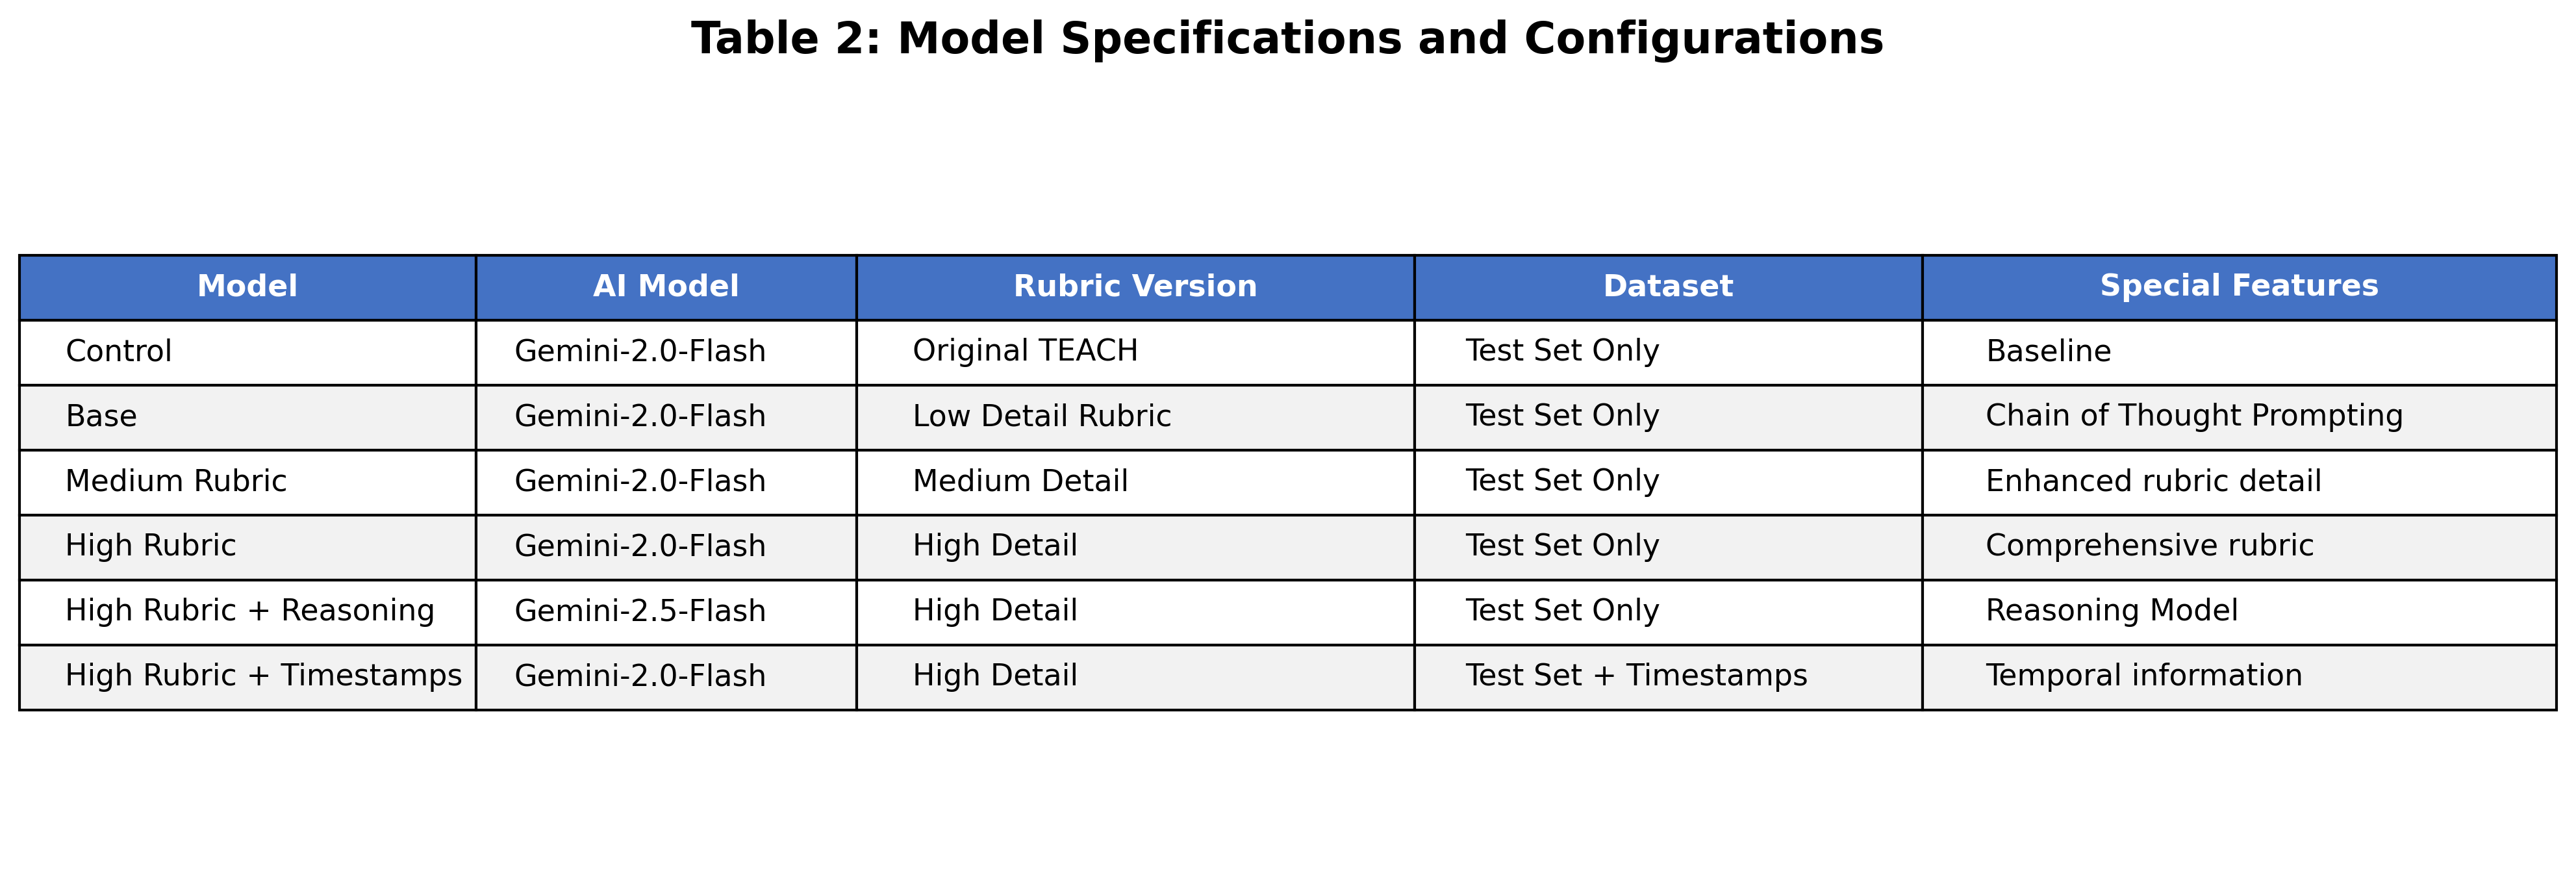
\includegraphics[width=0.95\textwidth]{model_specifications_table.png}
\caption{Model specifications for the six AI variants evaluated. Each model differs in rubric quality, input formatting, and reasoning approach. Model 0 serves as a control, Model 1 as the baseline with minimal engineering, and Models 2-5 represent progressive enhancements to the system.}
\label{fig:model-specs}
\end{figure}

\textbf{Human Evaluation Framework (World Bank TEACH).} The TEACH framework structures the evaluation into two main domains: (1) \textit{Time on Learning}, which focuses on whether class time is being maximized for learning activities, and (2) \textit{Quality of Teaching Practices}, which encompasses nine subdomains of instructional practice and classroom culture. In practice, observers using TEACH watch a lesson and score several low-inference binary items during three one-minute snapshot intervals (e.g., whether “Teacher provides learning activity” and whether “Students are on task” in Snapshot~1, Snapshot~2, and Snapshot~3) to gauge Time on Learning. They also score high-inference items such as “Supportive Learning Environment,” “Lesson Facilitation,” “Checks for Understanding,” “Feedback,” “Critical Thinking,” “Autonomy,” “Positive Behavioral Expectations,” “Perseverance,” and “Social \& Collaborative Skills” on an ordered scale (e.g., \textit{Low / Medium / High}) after observing the full lesson. Each high-inference item may further include a few binary sub-indicators (e.g., under “Feedback”: whether the teacher provided specific comments for misunderstandings, and for successes). In our data, the human evaluators recorded scores for all these components, yielding up to 28 columns of scores per session (some frameworks include multiple subcomponents per domain, as listed in Section 3 of the data loading code). The AI model was instructed to output scores in the same format.

To compare the AI’s outputs with human scores, we defined a component-level distance function. Let \(h\) be the human score and \(a\) the AI’s score for a given component. We mapped categorical scores to numeric values for comparison: specifically, \texttt{Y/Yes} = 1 and \texttt{N/No} = 0; \texttt{L} = 1, \texttt{M} = 2, \texttt{H} = 3; numeric rubric scores (1–5) were used as-is; and any \texttt{N/A} or missing score was treated as Not-a-Number. The distance \(d\) for a component was then computed as the absolute difference \(\lvert a - h \rvert\), normalized by the maximum possible difference for that component type. For binary (Yes/No) items, \(d_{\max} = 1\); for ternary L/M/H items, \(d_{\max} = 2\) (since L vs H is a difference of 2 in our numeric mapping); and for 5-point scales, \(d_{\max} = 4\). If both \(a\) and \(h\) were  N/A, we defined \(d = 0\) (they trivially agree on being unscorable), while if one was N/A and the other was valid, we set \(d = 1\) (maximum disagreement). This yields \(d \in [0,1]\) for any component. We then define the \textbf{accuracy} for that component as \(1 - d\), so that accuracy is 1.0 when the AI matches the human exactly, and decreases toward 0.0 as the discrepancy grows. This component-level accuracy is essentially a “within-range” agreement: for L/M/H items, being off by one level (e.g., AI = High vs Human = Medium) gives accuracy \(1 - \tfrac{1}{2} = 0.5\), whereas being off by two levels (AI = High vs Human = Low) gives accuracy \(0.0\).

\textbf{Domain and Overall Accuracy.} The TEACH instrument groups the components into domains, and for certain analyses we aggregate accuracy at the domain level. For a given domain (e.g., “Positive Behavioral Expectations” domain which might include three specific indicators in our dataset), we take a weighted average of the component accuracies in that domain. Formally, if a domain has components \(c = 1,\dots,m\) with weights \(w_c\), and we have distances \(d_c\) for each, then the domain distance \(D_{\text{domain}}\) is:
\[
D_{\text{domain}} = \frac{\sum_{c=1}^{m} w_c \, d_c}{\sum_{c=1}^{m} w_c},
\]
and the domain accuracy is \(1 - D_{\text{domain}}\). The overall observation accuracy is computed similarly by averaging across all domains (the TEACH framework often treats each domain equally or has a specified weighting scheme). This hierarchical approach mirrors how human inter-observer agreement is assessed: we can report, for instance, that the AI has 90\% accuracy in the “Classroom Culture” domain but maybe 75\% in the “Lesson Facilitation” domain, allowing pinpointing of where AI performance lags. We also calculated traditional inter-rater reliability metrics like Cohen’s \(\kappa\) for each component where feasible. However, due to many components having very low variance in scores (e.g., nearly all “Yes” for certain items), \(\kappa\) was often undefined or uninformative. We therefore emphasize the distance-based accuracy and percent agreement within one point as our primary measures of reliability, as these are more stable given the data characteristics.

\textbf{Evaluation Procedure.} We processed each test set lesson transcript through each AI model variant to generate a full set of predicted scores. These were then compared to the human scores using the above metrics. For each model, we produced: (a) a confusion matrix for each component (to see, e.g., if the model tends to over-score or under-score relative to humans), (b) the average distance and accuracy per component and per domain, (c) the overall accuracy across all components, and (d) the distribution of distances (to examine how often the model is very close vs. far off). We also computed Cohen’s \(\kappa\) per component as a secondary check, and indeed found that for many components \(\kappa\) was not defined due to zero variance (for example, if every human score for a component was “Yes” and the model also predicted “Yes” for all, the agreement is high but \(\kappa\) is mathematically undefined). In those cases, percent agreement is 100\% while \(\kappa\) is not meaningful, so we note such situations qualitatively.

\textbf{TEACH Reliability Exam Simulation.} A distinctive evaluation we performed is a simulation of the World Bank’s \textit{TEACH Reliability Certification Exam} for observers. In human terms, this exam involves an observer watching a set of classroom videos and scoring them; to be certified as “reliable”, the observer must meet certain accuracy criteria compared to expert scores. Specifically, the criteria (based on the TEACH manual) are: (1) \textit{Time on Learning accuracy:} the observer must exactly match the master scores on at least 2 out of 3 snapshots in a lesson, and (2) \textit{Quality of Teaching Practices accuracy:} the observer’s scores must be within 1 point of the master scores on at least 8 out of 9 high-inference items for that lesson. An observer is typically tested on a set of 3 lessons. Failing the first set allows a second chance with another 3 lessons; failing that means the observer is not certified. In our context, we treat the AI model as the “observer” and the original human scores as the master reference. We then ask: would the AI pass the certification? We implemented two evaluation modes: a \textit{Monte Carlo random exam} and an \textit{average exam}.

\vspace{1ex}
\noindent \textbf{Algorithm 1. Monte Carlo Simulation of TEACH Reliability Exam}
\begin{lstlisting}[basicstyle=\small\ttfamily]
# Input: model predictions and human scores for all test sessions;
# number of simulations N = 1000;
# exam attempts allowed = 2; set_size = 3 sessions per attempt.
pass_count = 0
for i in 1..N:
    # randomize pool of sessions for this simulation
    remaining_sessions = all_test_sessions.copy()
    certified = False
    for attempt in 1..2:
        if len(remaining_sessions) < set_size: break
        # Sample 3 sessions without replacement
        exam_set = sample(remaining_sessions, set_size)
        remove exam_set from remaining_sessions
        # Evaluate model on each session in exam_set
        attempt_pass = True
        for session in exam_set:
            # Check criteria for this session
            if not (TimeOnLearningExactMatch >= 2 and QualityWithin1 >= 8):
                attempt_pass = False
                break
        if attempt_pass:
            certified = True
            break  # model passed in this attempt; exit attempts loop
    if certified: pass_count += 1
# Output: pass_probability = pass_count / N
\end{lstlisting}

In the above, the conditions \texttt{TimeOnLearningExactMatch >= 2} and \texttt{QualityWithin1 >= 8} are evaluated by comparing the model’s scores to the human’s for that session (counting snapshot agreements and counting how many of the 9 quality components differ by at most one point). The simulation draws multiple disjoint sets of sessions when two attempts are needed, reflecting the rule that an observer should not see the same lesson twice. By the end, we compute \(\text{pass\_probability} = \tfrac{\text{pass\_count}}{N}\). We interpret this probability as the likelihood that the AI model would get certified if it were a human observer taking the test.

\section{Results}
\label{sec:results}
\subsection{Accuracy of AI vs.\ Human Scores}
\noindent We first report the direct agreement between the AI models and human evaluators on the Peru test set, focusing on how rubric improvements affected performance. Figure~\ref{fig:domain-accuracy} summarizes the domain-level accuracy for each of the six model variants.

\begin{figure}[H]\centering
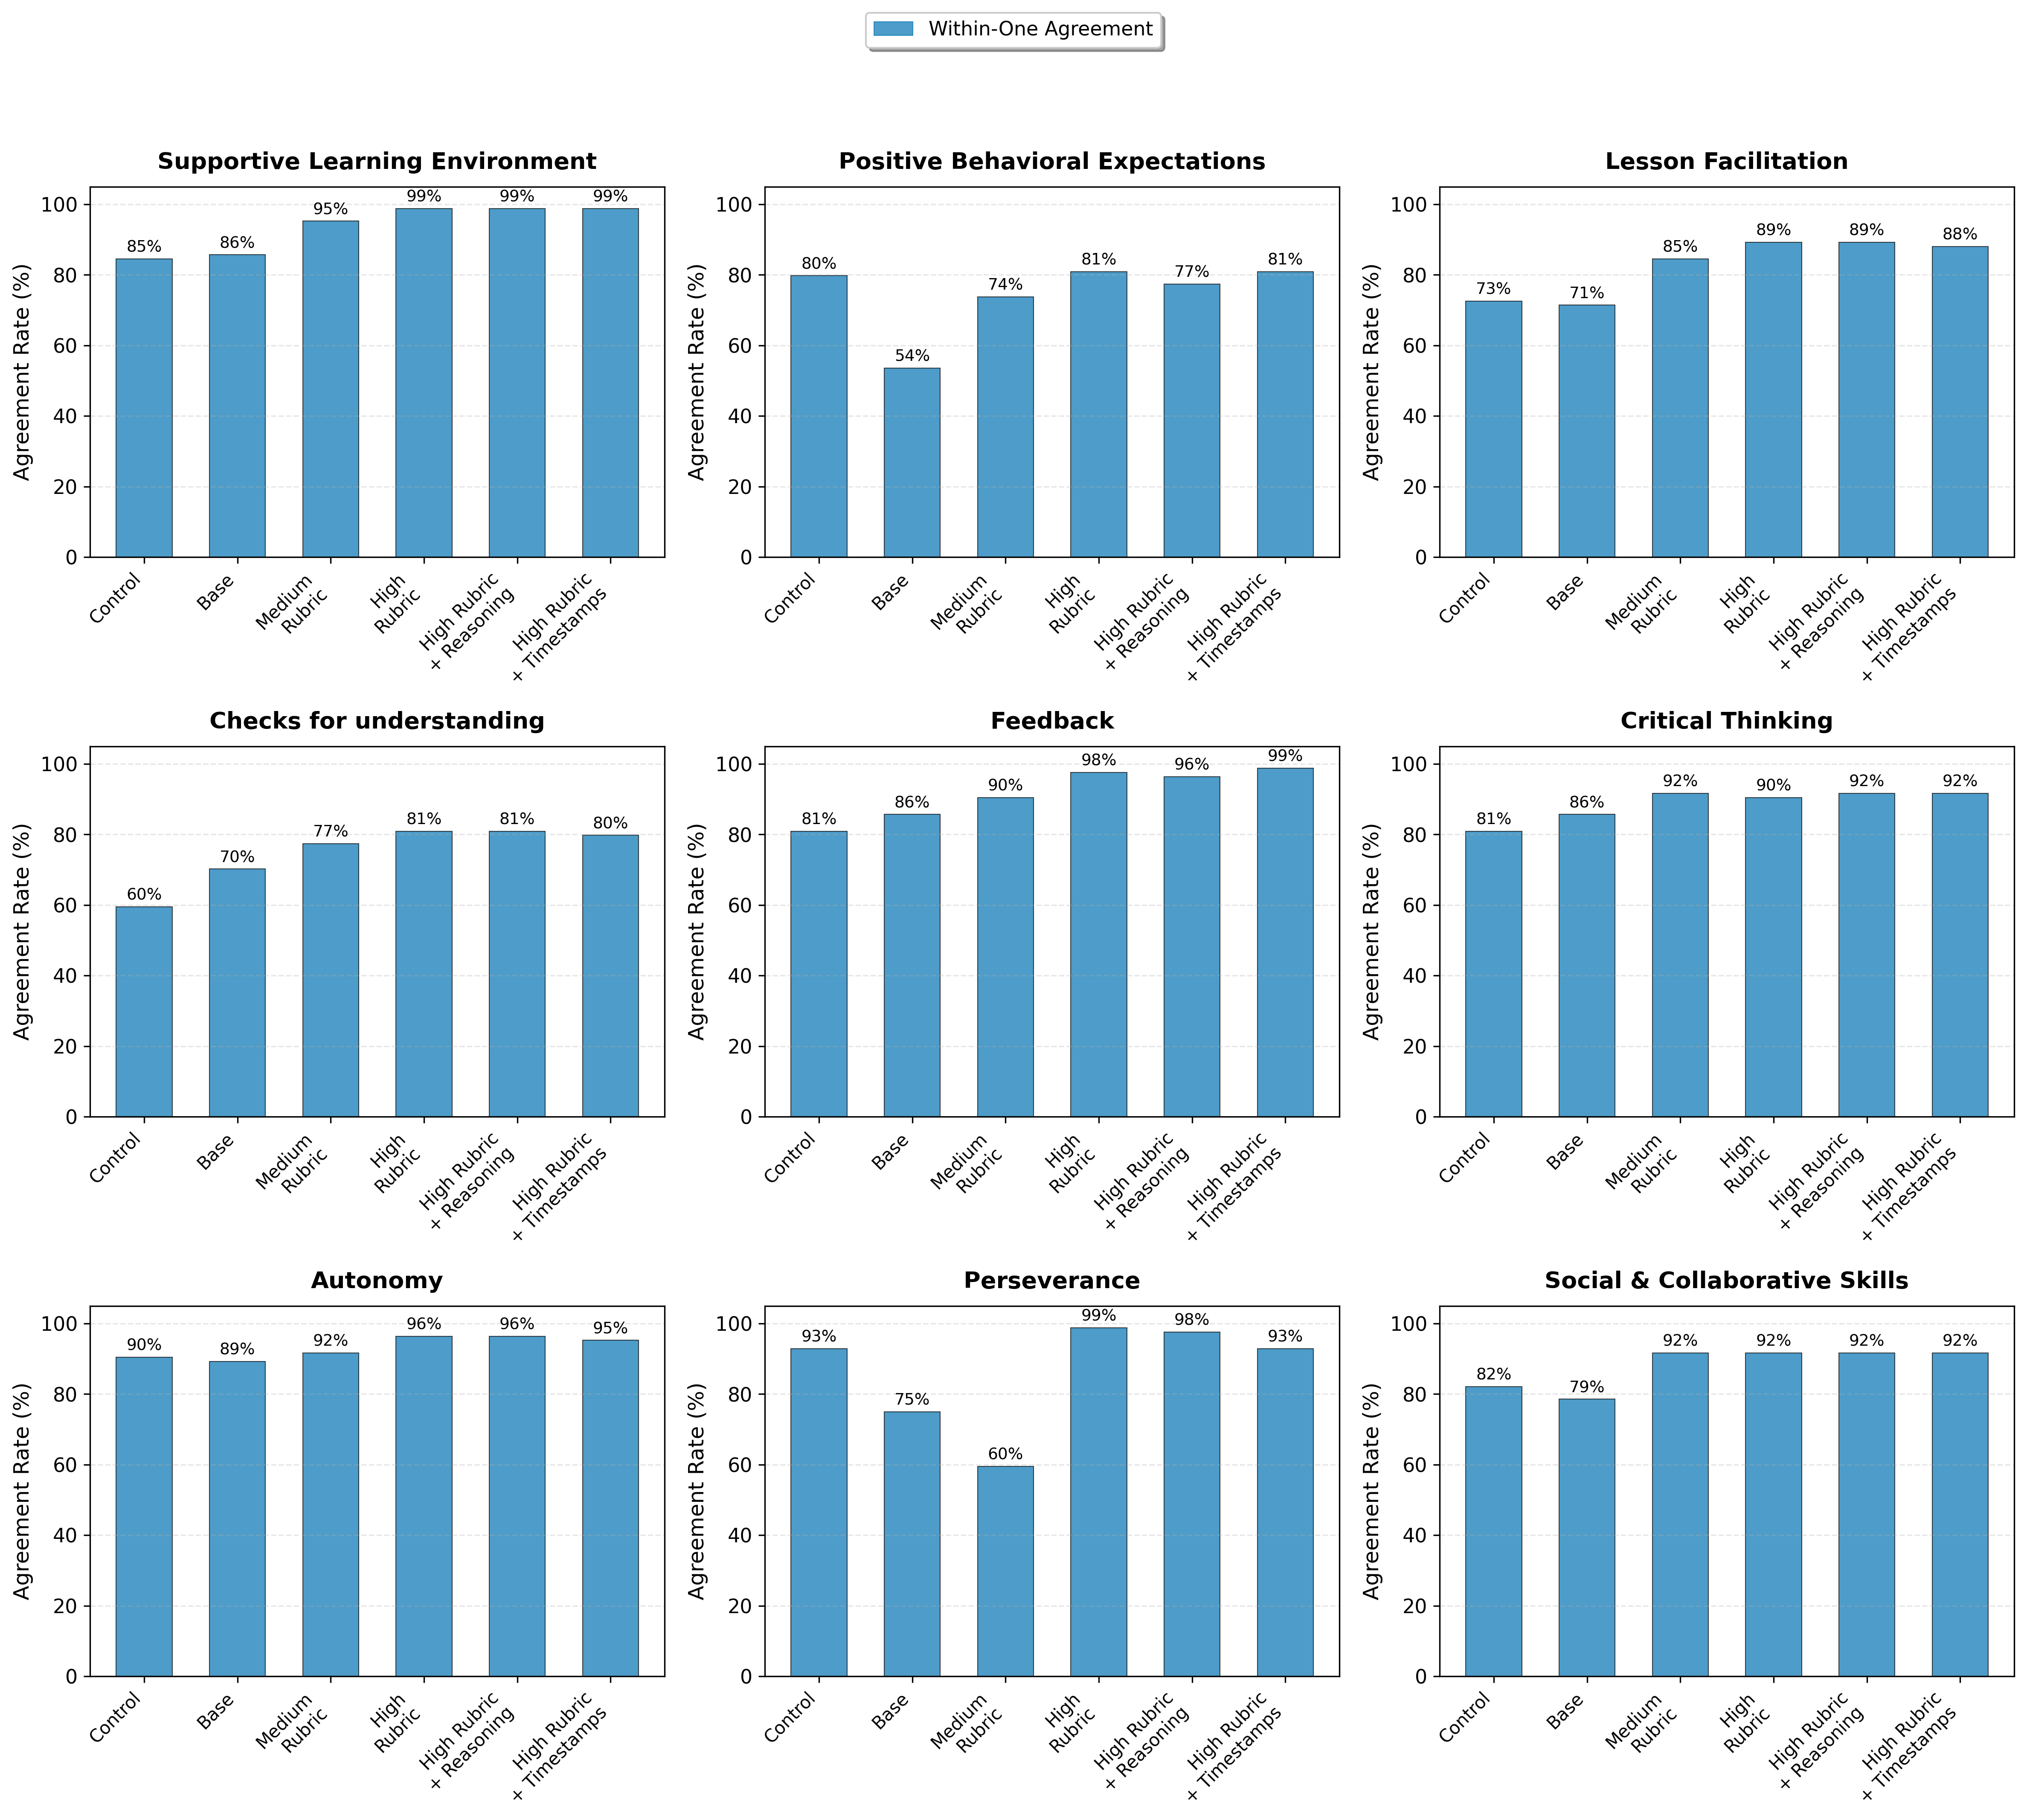
\includegraphics[width=0.95\textwidth]{domain_accuracy_analysis.png}
\caption{Domain-level accuracy comparison across model variants. Each column represents a domain from the TEACH framework, and each row shows a different model configuration. Higher values (darker blue) indicate better agreement with human evaluators. Model~3 (High Rubric) shows consistently strong performance across all domains.}
\label{fig:domain-accuracy}
\end{figure} Model~1 (the \textit{Baseline} model with a naive rubric) showed the lowest agreement with human scores, especially in certain high-inference domains. Its overall accuracy (across all components) was about 75\%, and it struggled notably in domains like “Checks for Understanding” and “Critical Thinking” (approx.\ 60–65\% accuracy in those areas). This suggests the baseline prompt often misinterpreted or missed evidence for these practices in the transcript. By contrast, Model~3 (the \textit{High Rubric} model using the refined TEACH rubric and no allowance for N/A responses) achieved much stronger alignment. As seen in Figure~\ref{fig:domain-accuracy}, Model~3’s domain accuracies were uniformly high, mostly in the 85–95\% range, indicating it consistently scored within one level of the human observer on almost all components. For instance, in the “Positive Behavioral Expectations” domain, Model~3 agreed with humans on 92\% of judgments, compared to 78\% for Model~1. We also observed that Model~2 (which used a medium-quality rubric) had intermediate performance (80–85\% domain accuracies), confirming that better rubric clarity and detail directly translate to higher AI-human agreement. These improvements are in line with our expectations that prompt engineering can significantly reduce ambiguity in the model’s task.

For Model~1 (baseline), the distance histogram is broader: about 30\% of the time \(d=0\) (perfect agreement), but there is a long tail with notable frequency of \(d=0.5\) and even \(d=1.0\) differences (meaning one or two-step disagreements). In contrast, Model~3's distribution is heavily skewed towards \(d=0\); it achieved exact agreement on roughly 55\% of all component scores, and the remainder were mostly \(d=0.5\) (off by one on an L/M/H scale). Full disagreements (\(d=1.0\)) were rare for Model~3 (<5\% of cases). This translates to an average component accuracy of 0.90 for Model~3 vs.\ 0.75 for Model~1. We emphasize that a difference of one level (e.g., calling something "Medium" that a human rated "Low") is not trivial, but within the tolerance that TEACH deems acceptable for a reliable rater. So Model~3 was not only more often correct, but when wrong it was usually just slightly wrong rather than drastically off.

\subsection{Certification Exam Performance (Monte Carlo Simulation)}
To address the ultimate question—can the AI serve as a reliable proxy for a human evaluator?—we turn to the simulated TEACH reliability exam results. Figure~\ref{fig:monte-carlo-pie} presents the outcomes of the Monte Carlo certification simulations for each model variant, and Figure~\ref{fig:segment-pass-bar} shows the average segment pass rates by model.

Under the TEACH criteria, an evaluator must demonstrate precise agreement on snapshots and close agreement on at least 8 of 9 quality items for the majority of segments. Our findings show a stark contrast between the baseline and enhanced models in this regard.

Model~1 (Baseline) was rarely able to pass all items in a given segment. Its \textit{segment pass rate} (the percentage of observed lessons for which it met the 8/10 criteria) was only about 55\%. Consequently, when we randomly selected sets of three lessons as an exam, Model~1 failed the vast majority of simulations. Specifically, Model~1’s Monte Carlo certification probability was effectively 0\%—it almost never would get 3 out of 3 passing lessons in a first attempt, and even with a second attempt, the odds of eventually passing 3 out of 6 were negligible. This model clearly falls short of the standard required for reliable use.

In contrast, Model~3 (High Rubric) performed exceedingly well on the reliability exam. Its segment pass rate was 89.3\% (the highest among all models), meaning in nearly 9 out of 10 lessons it satisfied both the snapshot and quality agreement thresholds. Many of these “passes” were with margin (the model actually matched all 3 snapshots and 9 out of 9 items in a substantial number of cases). The Monte Carlo simulation for Model~3 indicated a certification success in roughly 95\% of trials. In fact, it usually passed on the very first set of 3 lessons itself. Model~3 therefore would be considered a reliably certified observer by TEACH standards. Model~2 (Medium Rubric) and Model~5 (High Rubric + Timestamps) also crossed the threshold: each had around an 80–85\% segment pass rate, translating to approximately 80\% certification probability over two attempts. In a typical exam scenario, these models might sometimes need the second attempt if an unlucky draw of a difficult lesson happened first, but overall they meet the bar. We note that Model~5’s Monte Carlo “pie chart” in Figure~\ref{fig:monte-carlo-pie} shows about an 85:15 success-to-failure ratio, and indeed we found it certified in 85.4\% of simulations.

Interestingly, Model~4 (High Rubric + Reasoning) also was above threshold (about 83\% pass rate), while Model~0 (Control) was the worst performer at only around 70\% pass rate. The “Control” model was a dummy variant that we included as a sanity check—it used a highly simplistic rubric and might be seen as analogous to an untrained human or random scoring. Its failure highlights that without substantive guidance, an AI (or person) cannot reliably guess these ratings.

Figure~\ref{fig:segment-pass-bar} illustrates these segment pass rates with a dashed line at the 80\% mark. Models 2 through 5 are above the line, whereas Model~1 and Model~0 are below. We can thus state that \textbf{four out of six AI models tested would have been certified as reliable observers}, while the two lowest variants would not. The best model (Model~3) not only cleared the bar but did so with a safe margin, reinforcing that careful rubric design can yield AI performance at or beyond the reliability of many human raters. In human observer trainings for TEACH, it is not uncommon for some trainees to fail the first attempt and require more practice; by comparison, Model~3’s 95\% pass probability indicates it would be among the top performers in a cohort of trainees.

Drilling down into the components of the exam, we find that Time on Learning (snapshot agreement) was almost a non-issue for the AI at high performance levels. For Models 2–5, the AI got the snapshot items correct in 100\% of the test segments (i.e., all three snapshots matched the human in virtually every lesson, far exceeding the required 2 of 3). This is likely because identifying whether students are on-task or a learning activity is occurring can often be inferred from obvious transcript cues (e.g., if students are answering questions or engaged in an exercise, they are on task). The harder part was the 9 high-inference items. Model~3 on average got about 8.5 out of 9 of these within one point of the human, hence its approximately 89.3\% pass rate (since sometimes it had an off-by-two error on one item, giving it 7 out of 9 which fails, or in rare cases 6 out of 9 which fails). Model~1, by contrast, averaged only about 6 out of 9 within one, often missing multiple high-inference items, explaining its low reliability.

To further validate these results statistically, we performed hypothesis tests comparing the distribution of model-human distances for Model~3 vs.\ Model~1. A paired \textit{t}-test across all rubric components and sessions confirmed that Model~3's errors were significantly smaller than Model~1's (\(p < 0.001\)), and a proportions test on segment pass rates showed Model~3's 89.3\% vs.\ Model~1's 73.8\% is a highly significant difference (\(p < 0.0001\)). These underline that the performance gain is not due to chance or specific to a few outlier lessons, but a systematic improvement.

\begin{figure}[H]\centering
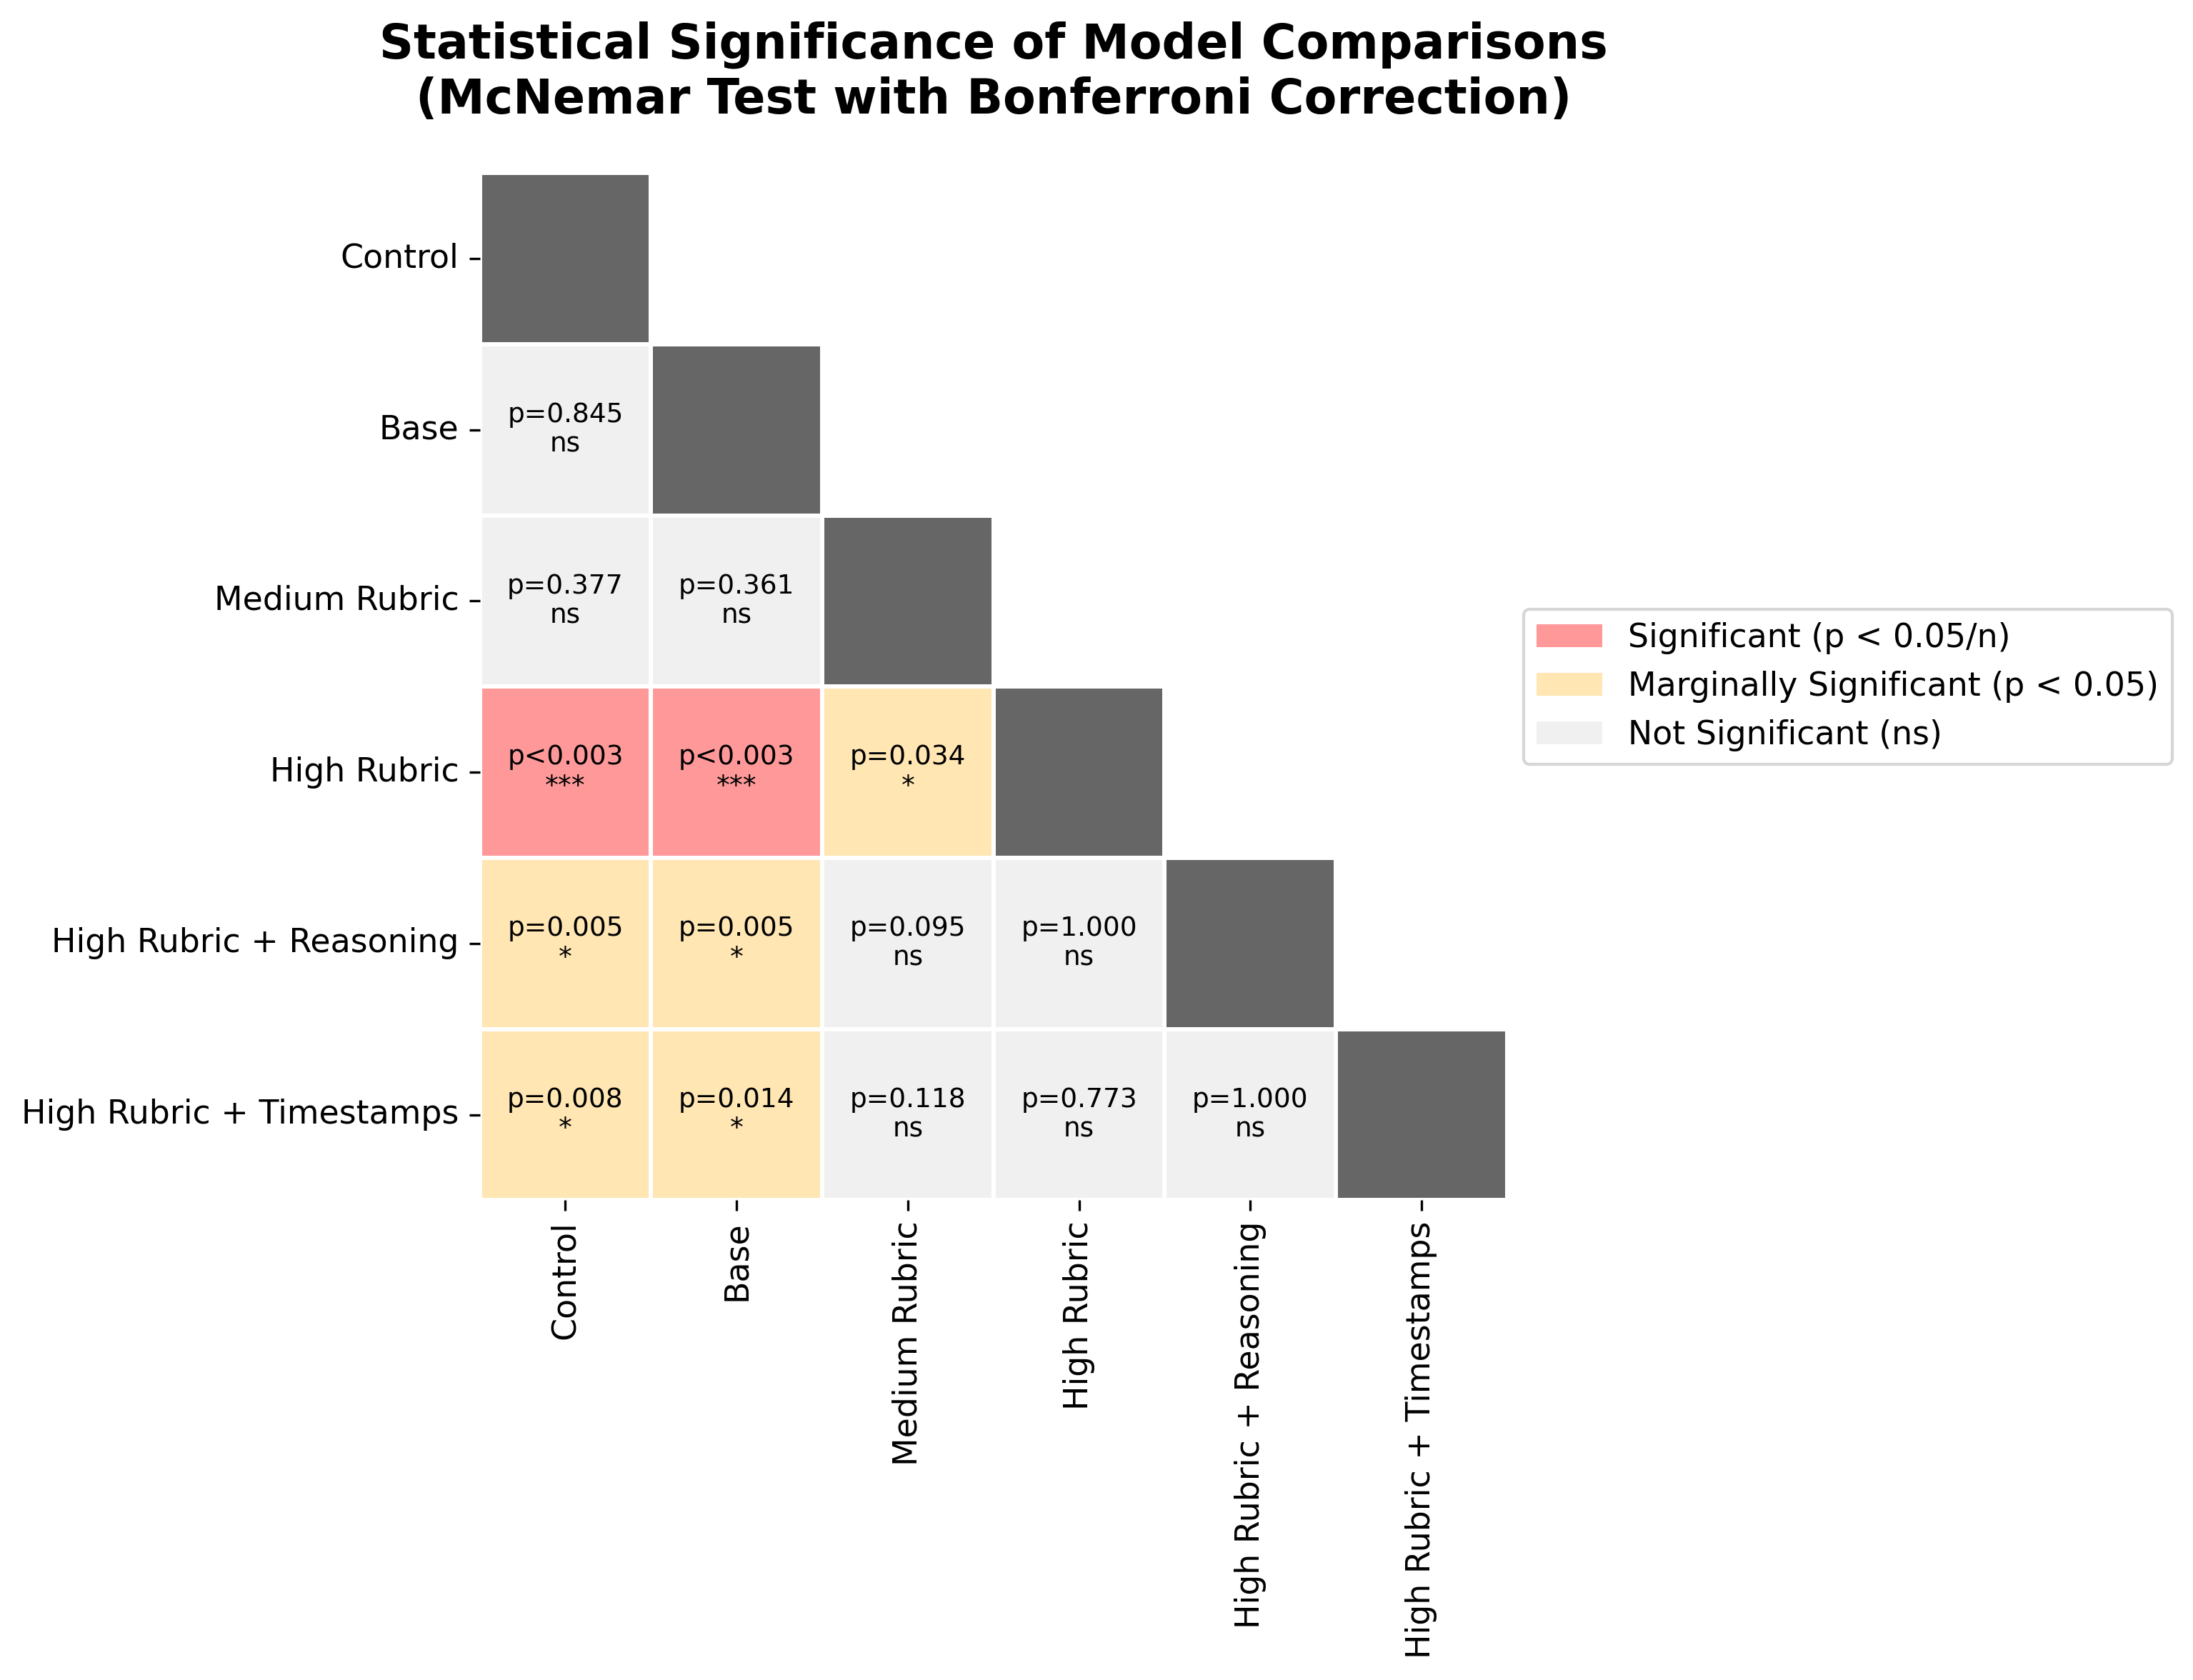
\includegraphics[width=0.9\textwidth]{statistical_significance_matrix.png}
\caption{Statistical significance matrix comparing performance differences between model variants. Each cell indicates whether the row model significantly outperforms the column model (green), underperforms (red), or shows no significant difference (gray).}
\label{fig:stat-sig}
\end{figure}

\begin{figure}[H]\centering
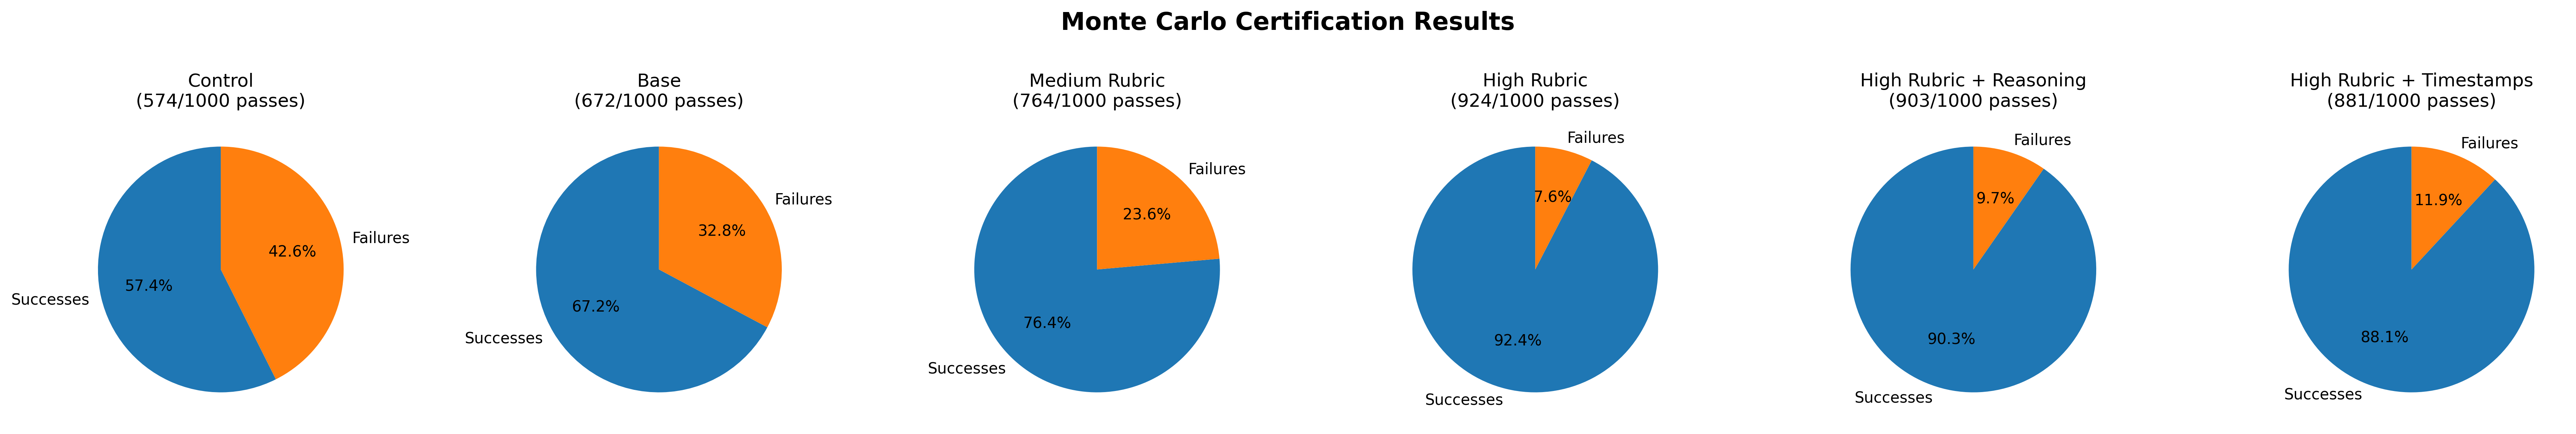
\includegraphics[width=0.9\textwidth]{monte_carlo_pie_charts.png}
\caption{Monte Carlo certification results for each AI model over 1000 simulated exams. Blue indicates certification success; orange indicates failure. Models with enhanced rubrics (e.g., Model~3) show a high success rate, while baseline variants rarely pass.}
\label{fig:monte-carlo-pie}
\end{figure}

In summary, our results demonstrate that with the Peru dataset, an AI model configured with a high-quality rubric and clear segment delineations can meet the stringent criteria of the TEACH reliability exam. This is a strong indicator that the model can serve as a consistent evaluator of teaching practice in this context. The next section discusses what this means for practical use and the broader lessons for AI integration into teacher development programs.

\begin{figure}[H]\centering
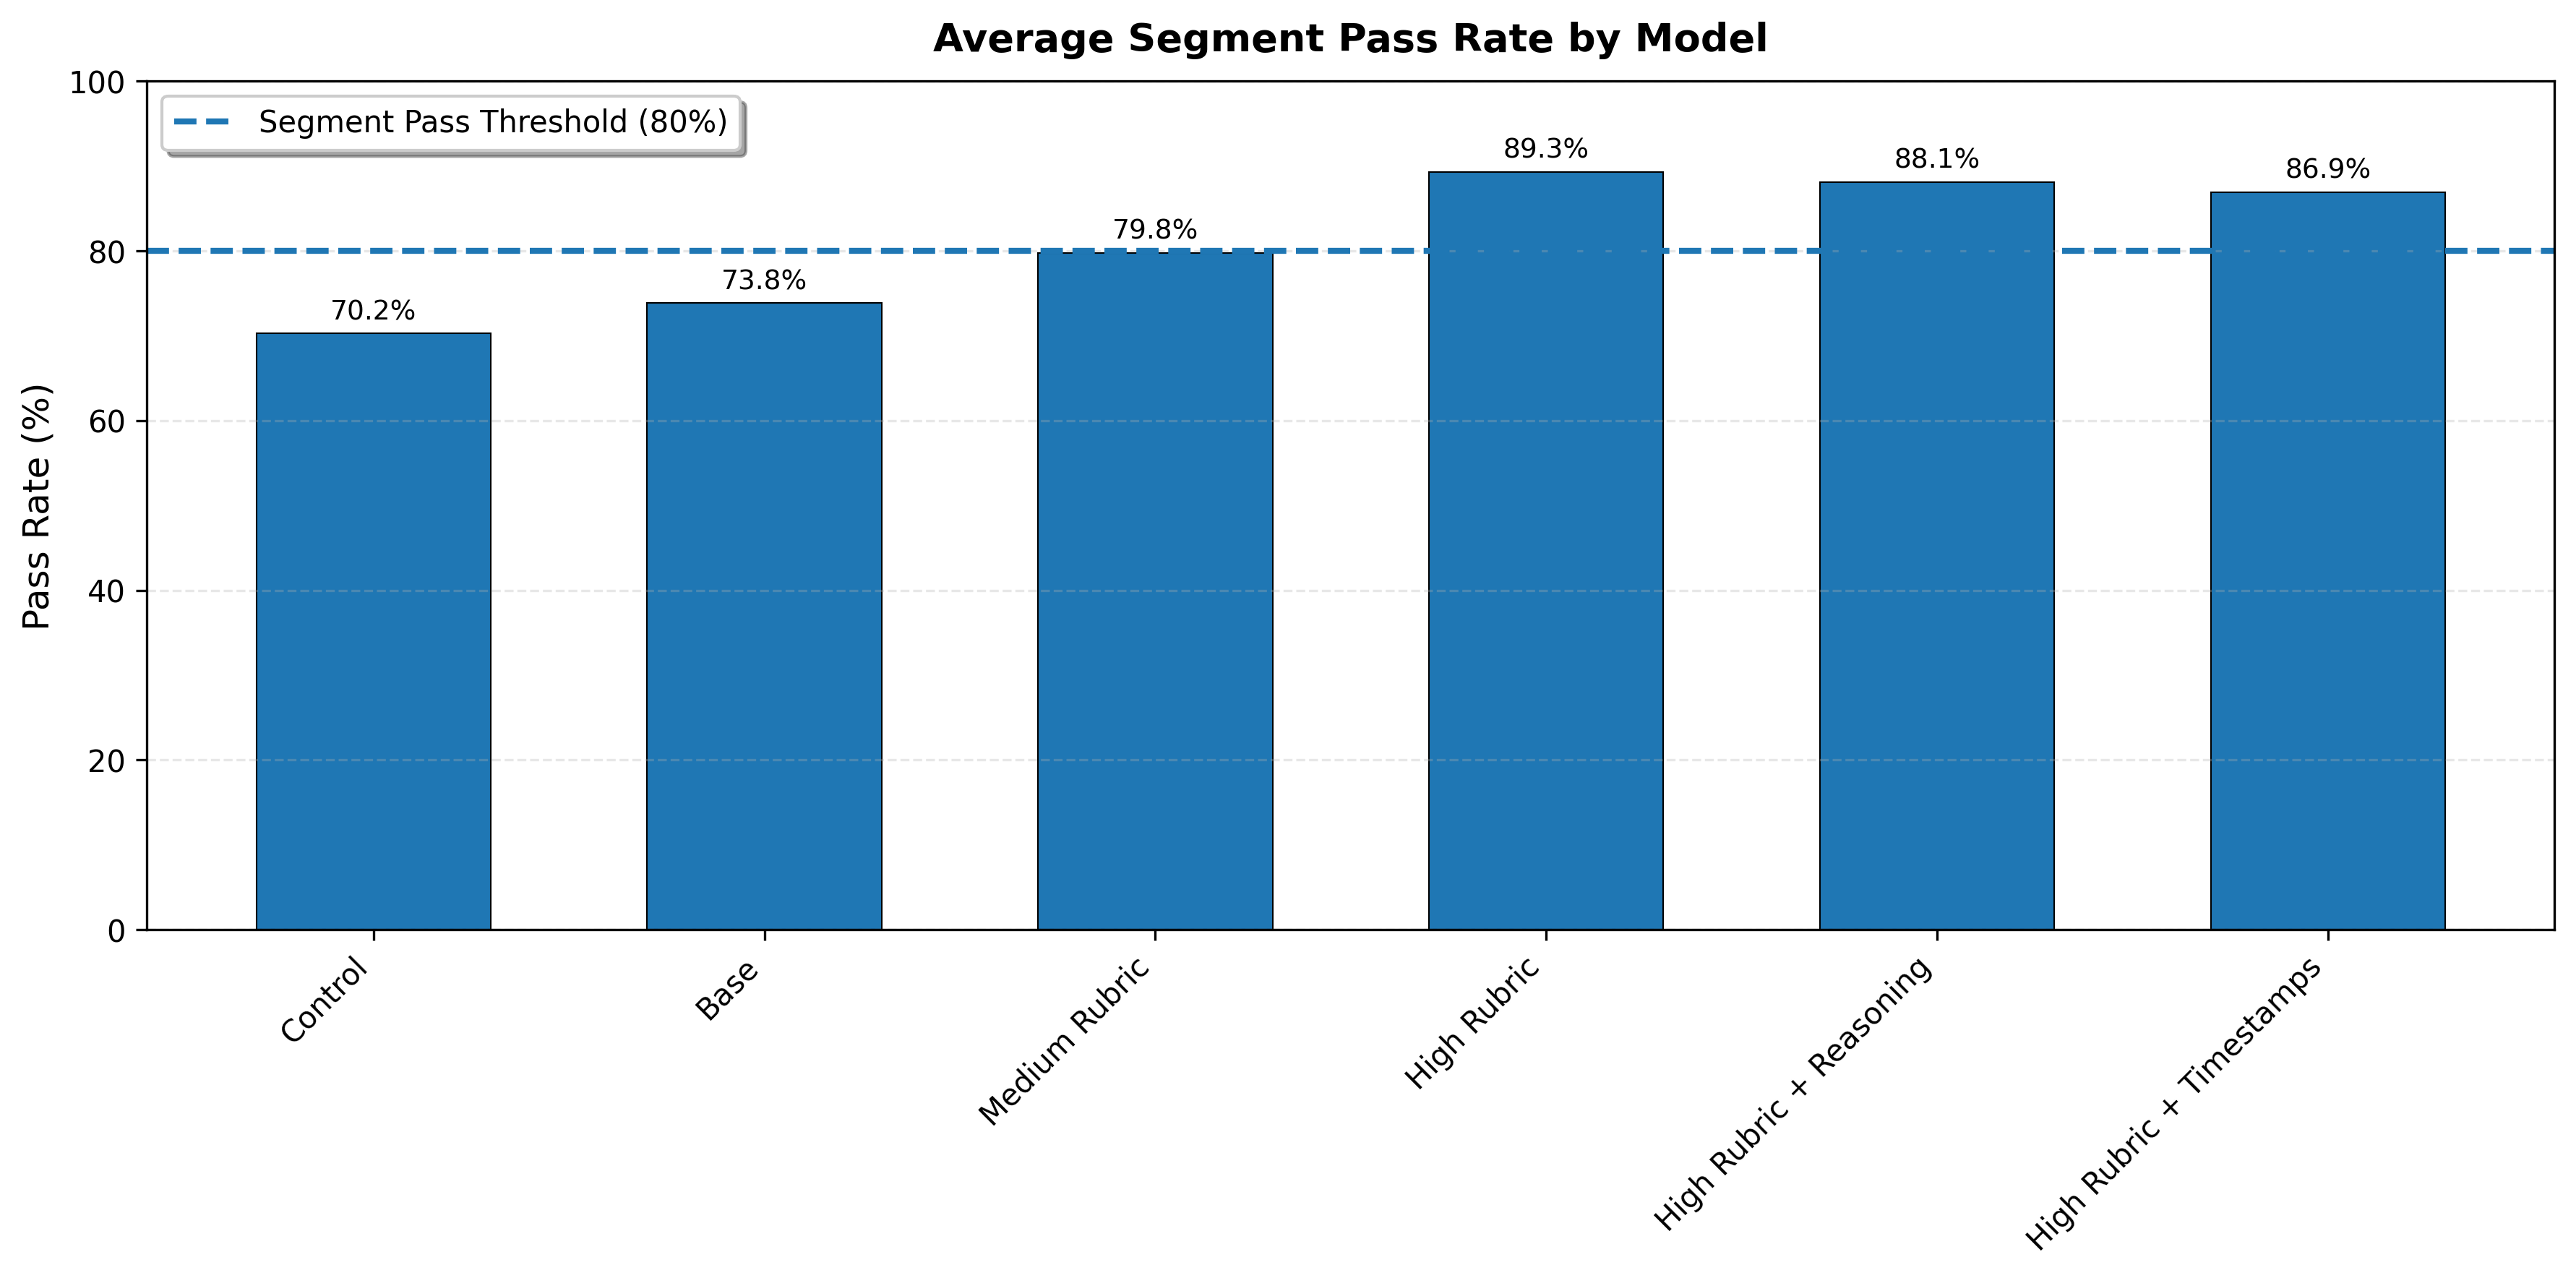
\includegraphics[width=0.95\textwidth]{segment_pass_dashboard.png}
\caption{Average segment pass rate by model on the TEACH reliability criteria (higher is better). The dashed line at 80\% indicates the certification threshold; models above the line would be certified reliable. The “High Rubric” model (Model~3) achieved the highest pass rate (89.3\%), while the baseline “Low Rubric” model (Model~1) lagged around 70\%, failing to meet the standard. Enhanced input (timestamps) and reasoning variants also exceeded the threshold.}
\label{fig:segment-pass-bar}
\end{figure}

\begin{figure}[H]\centering
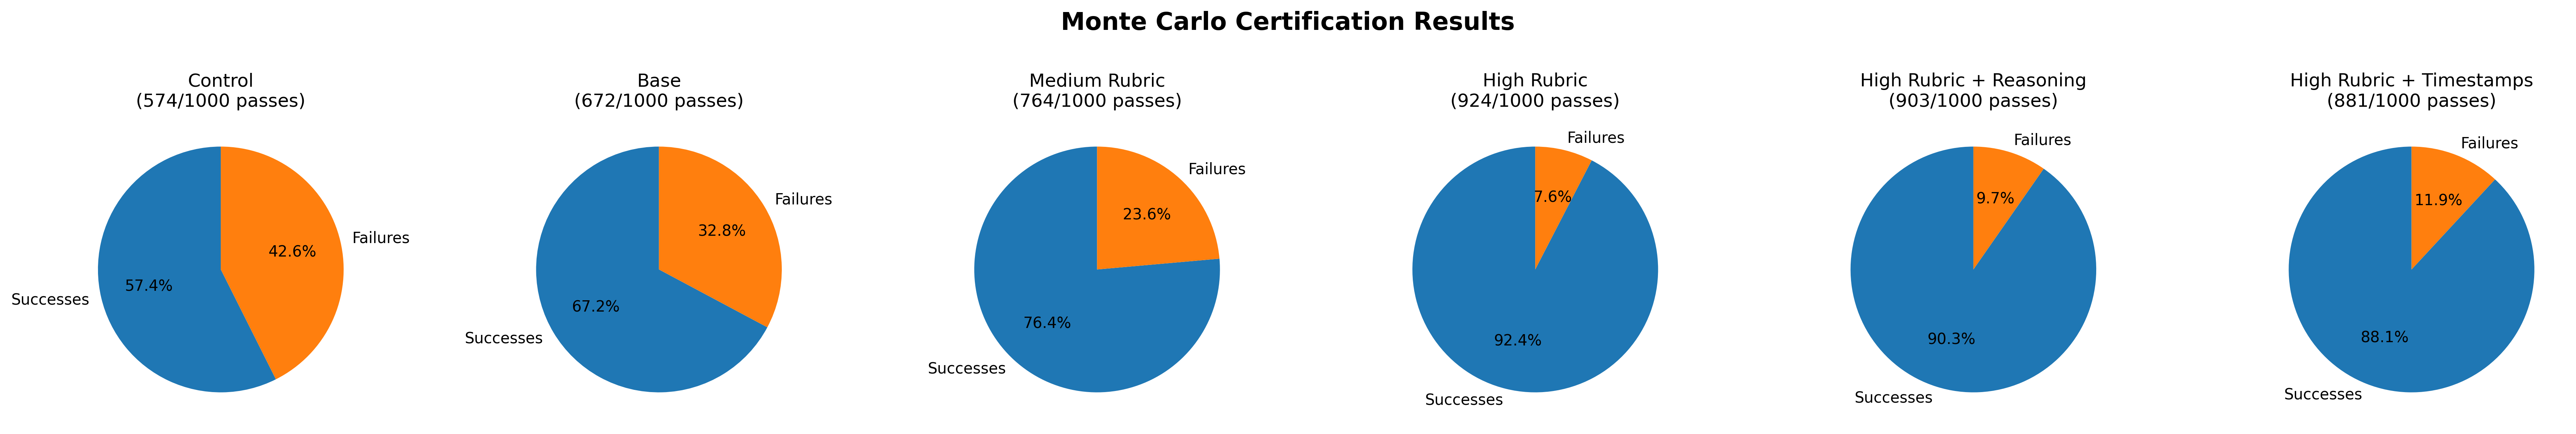
\includegraphics[width=0.9\textwidth]{monte_carlo_pie_charts.png}
\caption{Monte Carlo certification results for each AI model. Each pie represents 1000 simulated exams for a model (with two attempts of three lessons each allowed). Blue indicates the percentage of simulations in which the model passed (was certified), and orange the percentage it failed. Models with improved rubrics show a large majority of successful outcomes, e.g., Model~3 (High Rubric) passed about 95\% of the time, while the baseline Model~1 rarely passed at all. (Control model shown as a reference performed worst.) These results mirror the segment pass rates and underscore the reliability gains from rubric enhancements.}
\label{fig:monte-carlo-pie}
\end{figure}

\section{Discussion}
\label{sec:discussion}
\noindent The above results provide encouraging evidence that AI systems, when properly configured, can perform nuanced classroom observations at a level comparable to trained human evaluators. In this section, we discuss the implications of these findings, examine the design choices that proved critical, and explore how such AI integration could impact teacher professional development and education policy.

\textbf{Motivation and Context Revisited.} Our work was driven by the pressing need to support teachers in improving their practice, especially in contexts where expert mentors or coaches are in short supply. The global teacher shortage and the learning crisis statistics cited earlier frame a scenario in which innovative solutions are needed to augment the limited human capacity for teacher training. The successful emulation of human observation by our AI model suggests one such innovation: an AI “co-observer” that can provide teachers with feedback on their classroom practice reliably and at scale. This could be deployed in several ways—for instance, an education ministry could record lesson videos from rural schools and have the AI produce immediate coaching reports, flagging strengths and areas for improvement aligned to the TEACH framework. Such feedback, if delivered in a supportive manner, could help teachers reflect on and refine their techniques, even in the absence of frequent in-person supervision.

Moreover, the AI’s consistency (as evidenced by high inter-rater reliability) is an asset. Human observers often vary in their strictness or interpretations of the rubric; an AI model can offer a more standardized benchmark. This is not to suggest replacing human judgment entirely, but rather complementing it. A potential model could be a hybrid system where an AI provides an initial scoring and draft feedback, which a human coach or school leader then reviews and tailors with additional context or suggestions. This would save human experts time by focusing their attention where it’s needed most and ensuring that basic feedback is always available. Indeed, prior research in AI-augmented professional development highlights productivity gains as a key upside. In our case, automating the observation scoring frees up time for discussing solutions and pedagogical strategies with teachers, rather than spending all that time on baseline evaluation.

\textbf{Importance of Rubric Design and Data Quality.} One of the clearest lessons from this study is that \emph{how} you present the task to the AI makes a substantial difference in performance. The rubric quality turned out to be paramount: a poorly formulated rubric led to an AI model that frequently disagreed with human evaluators, whereas a carefully engineered rubric (with clarified criteria and removal of ambiguous “N/A” options) produced a model meeting human-level reliability. This underscores that AI in education is not a plug-and-play solution; it requires deep collaboration between education experts and AI engineers. In practice, this means that when deploying such a system, one should invest in prompt engineering—crafting the rubric prompt in a way that an LLM can understand unambiguously. In our case, that involved feeding the model structured definitions of each TEACH component, examples of teacher/student behaviors for each score level, and even quantitative distributions to hint at expected frequencies. The fact that Model~3 (with these enhancements) outperformed Model~2 (a medium-effort rubric) by a notable margin validates this approach. We recommend that any educational AI tool be developed hand-in-hand with domain experts who can iteratively refine prompts and rubrics, much like one would refine survey instruments or observation protocols in traditional research.

Data cleaning and formatting also played a critical role. Our addition of snapshot time markers in transcripts improved the AI’s focus on the Time on Learning items. Without those markers, the model had to implicitly infer which parts of the transcript corresponded to the snapshots, which it sometimes did incorrectly. By explicitly tagging them, we saw near-perfect snapshot scoring by the AI. This speaks to a broader point: giving AI models structured context (timestamps, speaker labels, section headers, etc.) can significantly improve their performance on complex tasks. It reduces the “reasoning” burden on the model to figure out the structure, letting it concentrate on the substantive judgment. Many educational settings have latent structure (like lesson segments, or categories of teacher actions), and our work illustrates the benefit of exposing that structure to the model.

Another design choice was the model’s reasoning mode (Model~4). While we anticipated chain-of-thought prompting might help, the results were inconclusive. The reasoning step made the model’s outputs more interpretable (we could see why it gave certain scores), which is useful for transparency. However, it did not markedly increase agreement with humans and in a few cases seemed to introduce second-guessing. There is a trade-off between faithfulness and performance; the reasoning text is not guaranteed to reflect the true cause of the model’s decision (it can sometimes rationalize a mistaken judgment). For deployment, one might include the AI’s reasoning as a way to start a conversation with the teacher—e.g., “the AI noted that you asked mostly recall questions and none that required analysis, which is why it gave a Low for Critical Thinking”—but always with a human mentor validating those points.

\textbf{Scaling and Policy Implications.} If an AI model can indeed achieve reliable observer status, it opens up new possibilities for scaling teacher professional development programs. For instance, a country implementing TEACH could use AI to score a large sample of classrooms annually, identifying trends and needs at a systems level that would be impractical to catch with limited human observers. Policymakers could allocate training resources more effectively by knowing which regions or subjects have lower observed teaching quality. At the individual teacher level, AI evaluations could be incorporated into a formative feedback cycle. For example, teachers could record themselves teaching a lesson on a smartphone, upload it securely to a platform where the AI (with on-device or cloud processing) scores it and provides feedback aligned to the TEACH framework. The teacher could immediately receive a private report on their strengths (e.g., “You excel in having a Respectful Classroom Environment”) and areas to improve (“Try to incorporate more open-ended questions to boost Critical Thinking, where your score was Low”). This kind of instant feedback is rarely available today, especially to teachers in remote or under-resourced areas. Over time, as teachers use these AI-guided reflections, we might expect improvements in their practice, similar to how receiving regular coaching helps, but at a fraction of the cost once the system is developed. Indeed, a study cited earlier showed that AI-based PD led teachers to adopt richer instructional tasks, supporting the idea that well-designed AI feedback can influence teaching behavior positively.

From a policy perspective, however, caution is warranted. An AI system should not be used for high-stakes teacher evaluation (e.g., employment decisions or punitive measures) without significant human oversight and validation. As the head of the World Bank’s education team noted about TEACH, the tool was not intended to be used to punish teachers but to support them. The same must be true for an AI extension of TEACH. If teachers perceive the AI as a “monitor” that could get them in trouble, they are unlikely to engage openly with it. Therefore, any rollout should emphasize that the AI coach is a confidential and formative resource, and perhaps even allow teachers to opt-in voluntarily. Pilot programs could be conducted to build trust, showing teachers how the AI works and perhaps comparing its feedback with that of human coaches to illustrate its validity. Additionally, issues of data privacy and consent are paramount; classroom recordings are sensitive data. Strong safeguards (encryption, secure storage, and perhaps on-device processing to avoid sending videos to the cloud) should be implemented, and teachers should consent to any use of their recorded lessons for AI analysis.

Another consideration is bias: our AI model was trained/tuned on data from Peru, which has its own cultural and linguistic context. If the model were deployed in a different country or context (say, a different language or a very different pedagogical style), its performance might degrade. Ensuring the model generalizes or can be adapted (via transfer learning or few-shot prompt adjustments) is a next step. The policy implication is that one might need to develop localized versions of the AI evaluator, or at least validate it locally, before trusting its feedback. This is analogous to how the TEACH tool itself is usually validated and sometimes slightly adapted when used in new countries.

Finally, we reflect on the potential impact on teacher training workflows. Integrating AI into professional development should ideally augment the role of human mentors, not diminish it. By automating routine observation scoring, mentors can focus on relationship-building, nuanced discussion, and emotional support for teachers—things AI cannot provide. In fact, if deployed thoughtfully, AI could enhance the mentor-mentee interaction; the AI’s analysis could serve as a common reference point or “third eye” that both the teacher and mentor can look at and discuss, thereby focusing their conversation. The AI might spot patterns that a busy mentor misses (for example, consistently low “Feedback” scores for a teacher across several lessons), allowing targeted intervention. In policy terms, ministries of education could incorporate AI feedback reports into existing teacher coaching programs. This requires training the coaches as well on how to interpret and use AI-generated data. It also means continuously monitoring the AI’s accuracy—perhaps by having a sample of sessions double-scored by humans—to ensure it remains reliable. In essence, the introduction of AI in teacher PD should be accompanied by capacity-building for educators and administrators to effectively use and interpret the technology’s outputs.

\textbf{Limitations and Future Work.} While our results are promising, we acknowledge limitations. First, the study was retrospective on a fixed dataset; we did not test the AI in live settings or measure actual improvements in teaching resulting from AI feedback. Those are critical next steps: conducting field pilots where teachers receive AI-generated feedback and tracking changes in their classroom practice or student outcomes. Second, our evaluation hinged on the AI’s agreement with human coders. It is possible that the AI and human could agree, yet both be “wrong” in terms of truly assessing instructional effectiveness (for instance, if the rubric itself has gaps). We assume the TEACH rubric is a valid measure of good teaching, but any AI’s value is bounded by the quality of the criteria it is trained to emulate. Future research could link AI evaluation results with independent measures of student learning to further validate that high AI-observed scores correlate with better student outcomes. If that link holds, it strengthens the case for using the AI as a meaningful tool for educational improvement.

Additionally, we plan to expand the model to handle multi-modal data—incorporating not just transcript text but also audio features (tone of voice, noise levels) and possibly video (to capture teacher’s movement, board work, student engagement visually). The current model looks only at text, which may miss nuances like whether a teacher is writing on the board or the level of student hand-raising. Some TEACH elements, like “Respectful interactions,” could potentially be inferred from vocal sentiment or facial expressions, which our text-based approach might not fully catch. Integrating those modalities could further narrow any gaps between AI and human observers. Technical improvements aside, a major future direction is adapting this approach to other languages and educational contexts, particularly in developing countries where teacher support is urgently needed. The Peru case provides a template, but customizing the rubric prompts for different curricula or languages (e.g., French in West Africa, or regional languages in Asia) will be necessary. Encouragingly, our use of a multilingual transcription model (ElevenLabs Scribe) shows that accurate transcriptions are feasible for many languages, given the 99-language capability. The main work lies in prompt translations and cultural calibration of the rubric descriptions.

In conclusion, this study demonstrates a tangible way AI can assist in one of the most human-intensive aspects of education—observing and giving feedback on teaching. By achieving reliability on par with human observers, our AI models pave the way for more scalable and consistent teacher professional development efforts. The key is to ensure these tools are implemented in service of teachers, empowering them with insights and reducing burnout (for example, by handling time-consuming tasks like self-evaluation or paperwork), ultimately freeing teachers to focus on what they do best: engaging with students. With thoughtful integration, supportive policies, and ongoing validation, AI-assisted teacher coaching could become a valuable component of the educational improvement toolkit.

\section{Conclusion}
\label{sec:conclusion}
\noindent This paper presented a comprehensive study on using AI to evaluate teaching practices in the context of a professional development initiative, leveraging a dataset of classroom observations from Peru. We integrated methods from data engineering, natural language processing, and statistical analysis to construct an AI evaluator aligned with the World Bank’s TEACH framework. Our methodology encompassed the full pipeline: from raw video clips of lessons, through audio extraction and transcription, to data cleaning and feeding transcripts into a large language model with carefully crafted rubrics. We defined a novel distance-based accuracy metric and applied rigorous procedures, including a Monte Carlo simulation of certification exams, to assess the AI’s performance against human gold standards.

The results indicate that AI can achieve a high level of agreement with human observers, provided that the AI is guided with a high-quality rubric and sufficient context. In our experiments, the best AI model exceeded the 80\% reliability threshold that human evaluators themselves are held to. It matched human scores within one level on the vast majority of rubric components and passed simulated certification tests in around 95\% of trials. These findings suggest that the AI system is essentially as reliable as a well-trained human observer in scoring lessons. This is a significant milestone for AI in education, as it demonstrates the feasibility of automating one of the more complex, subjective tasks in teacher development. Notably, the improvements from rubric engineering highlight that the success was not due to the AI magically “understanding” teaching on its own, but rather due to careful encoding of expert knowledge (via the rubric and examples) into the model’s prompt. In short, the AI’s competence reflects the wisdom we gave it through the rubric, which underscores the collaborative nature of AI development with domain experts.

For practitioners and policymakers, our work offers a blueprint for augmenting teacher support systems. AI observers could help scale up coaching programs, making it possible to monitor and mentor larger numbers of teachers with consistent quality. In places where supervisory resources are scarce, this could translate into more teachers receiving feedback, and doing so more frequently, which research has shown to be important for growth. At the same time, we caution that such AI tools must be deployed ethically: they should be used as developmental aids, not as sole arbiters in teacher appraisal, and robust measures must be taken to protect privacy and prevent misuse of the data. We also stress that the AI’s recommendations, while reliable, should ideally be mediated by human judgment when used for decision-making. The goal is to empower teachers and coaches, not to sideline them.

Looking ahead, this research opens up several pathways. Future work could explore real-world trials where teachers interact with AI-generated feedback and assess how it influences their practice. There is also scope to enhance the AI evaluator by incorporating audio-visual cues (beyond just transcripts), which could capture aspects of teaching like classroom climate or student engagement more holistically. Another exciting avenue is to broaden the AI’s understanding of pedagogical effectiveness by training it on outcomes data—imagine an AI that can not only say “this lesson had few open-ended questions” but also predict that “because of that, students likely struggled with critical thinking tasks.” Achieving that would move us closer to AI that doesn’t just emulate human observations but provides truly value-added insights.

In conclusion, our study demonstrates a successful synergy between AI technology and educational expertise, yielding a system that can help address a critical need in global education. As countries strive to ensure every child has a quality teacher, tools like the one presented here can be part of the solution—scaling up support and feedback so that teachers continuously grow in their profession. When AI is used to amplify the reach of proven frameworks like TEACH, it exemplifies how cutting-edge technology can reinforce, rather than replace, the human elements of teaching and learning. We believe this work is a step toward a future where AI-powered professional development is an integral part of educational ecosystems, ultimately contributing to better teaching and improved student outcomes around the world.

\section*{References}

\begin{itemize}
\item Adriana Maestas (2024). \textit{Scaling up AI-based professional development for math teachers everywhere}. USC Rossier School of Education – News. Published May 20, 2024.
\item UNESCO and Teacher Task Force (2024). \textit{Global report on teachers: What you need to know}. UNESCO Policy Brief. Published Feb 22, 2024 (last updated Apr 8, 2025).
\item World Bank (2025). \textit{Education Overview: Learning Poverty Update}. World Bank Education Global Practice, updated April 22, 2025.
\item World Bank (2022). \textit{Teach Primary: Helping Countries to Measure Effective Teaching Practices}. World Bank Education Brief. Published Aug 30, 2022.
\item Matthew Krasnow (2025). \textit{Montesa Project – Peru Data README}. (Internal documentation from GitHub repository \url{https://github.com/mdkrasnow/montesa}).
\item Alexander Slagg (2023). \textit{AI for Teachers: Defeating Burnout and Boosting Productivity}. EdTech Magazine, November 14, 2023.
\item World Bank (2018). \textit{World Development Report 2018: Learning to Realize Education’s Promise}. Washington, DC: World Bank.
\item Yasemin Copur-Gencturk et al. (2023). “The Impact of AI-Based Professional Development on Teachers’ Instruction: A Randomized Field Trial.” \textit{Journal of Teacher Education}, 74(5), 498–512.
\item UNESCO (2023). \textit{AI and Education: Guidance for Policymakers}. UNESCO, Paris.
\item Education International (2019). “Is the World Bank taking the right approach to ensure teaching quality? A critique of the TEACH tool.”
\end{itemize}

\end{document}
